\renewcommand{\tablename}{Cuadro}
Los resultados correspondieron a simulaciones a 3 GHz en cuatro medios. Se compararon primero las corridas a 5 px/mm y se utilizaron las resoluciones adicionales para examinar el efecto del refinamiento. Los perfiles radiales, las figuras y los informes de ajuste se consultaron en el material documentado en el \hyperref[an:fdtd-fuentes]{Anexo A}. El sufijo numérico de cada archivo indicó la resolución en píxeles por milímetro. Para las corridas que sólo contaron con una figura, se recuperaron los intervalos del informe asociado a la versión de la imagen.

\section{Incertidumbre de la atenuación y comparación entre medios}
Se estimó la atenuación aparente, $\alpha_{\mathrm{app}}$, a partir del perfil radial del flujo compensado por $r^2$. El programa de extracción documentado en el \hyperref[an:fdtd-fuentes]{Anexo A} calculó la componente radial a partir de $E_z$ y $H_\phi$ en la línea $z=0$. Se ajustó en decibelios el perfil de $|S_r|$ compensado por $r^2$. Se seleccionaron los puntos por encima de $-80$ dB entre $1.5\lambda$ y $4\lambda$ en vacío y concreto, y entre $2\lambda$ y $4\lambda$ en agua salada y músculo. Se exigieron $R^2>0.85$ y un RMSE inferior a $0.5$ dB para considerar utilizable el ajuste. Se intentaron 1500 reajustes por bloques de residuos con semilla cero y se tomaron los percentiles 2.5 y 97.5 de las estimaciones convergentes. Se reportó el intervalo de confianza (IC) del 95\,\% obtenido por remuestreo de bloques de residuos de cada ajuste. Este intervalo caracterizó la variabilidad de la pendiente dentro de la ventana radial utilizada. La discrepancia con la teoría se calculó por separado mediante $100|\alpha_{\mathrm{app}}-\alpha_{\mathrm{teo}}|/|\alpha_{\mathrm{teo}}|$ para los medios con pérdidas. En vacío se empleó la diferencia absoluta porque la referencia fue cero.

\begin{table}[htbp]\centering\small
\caption{Atenuación a 5 px/mm. Las atenuaciones y los límites del IC se expresaron en dB/mm. Las discrepancias porcentuales se tomaron de los informes de corrida.}\label{tab:fdtd-base}
\begin{tabular}{lcccc}\hline
Medio & $\alpha_{\mathrm{app}}$ & IC del 95\,\% & $\alpha_{\mathrm{teo}}$ & Discrepancia \\ \hline
Vacío & 0.0000 & $[0.0000,0.0075]$ & 0 & $0.0000$ dB/mm$^{*}$ \\
Concreto & 0.0380 & $[0.0380,0.0381]$ & 0.0385 & 1.31\,\% \\
Agua salada & 0.7012 & $[0.7005,0.7019]$ & 0.7326 & 4.29\,\% \\
Tejido muscular & 0.4669 & $[0.4663,0.4674]$ & 0.4921 & 5.12\,\% \\ \hline
\end{tabular}
\par\smallskip\footnotesize $^{*}$Se obtuvo este valor con un ajuste que incumplió el criterio de calidad.
\end{table}

El agua salada presentó la mayor atenuación, seguida del tejido muscular y del concreto. En los tres medios, la atenuación ajustada quedó por debajo de la referencia teórica y ésta quedó fuera del intervalo del ajuste. Los errores cuadráticos medios expresados como raíz (RMSE) fueron 0.0120, 0.0116 y 0.0063 dB, respectivamente. Los residuos conservaron estructura espacial, con estadísticos de Durbin--Watson de 0.0051, 0.0034 y 0.0008. Por ello, la precisión indicada por los intervalos dependió de la longitud de bloque utilizada y de la selección de la ventana de ajuste.

En vacío, el perfil compensado presentó oscilaciones intensas. Aunque se obtuvo una pendiente de 0.0000 dB/mm a la precisión registrada, el ajuste produjo $R^2=0.0000$ y un RMSE de 5.8227 dB. Se impuso $\alpha_{\mathrm{app}}\geq 0$ durante el ajuste y el remuestreo. La estimación quedó en el límite inferior a la precisión registrada. En vista de la dispersión observada y del criterio de calidad incumplido, la coincidencia con la referencia teórica resultó insuficiente para validar la extracción en vacío.

\section{Perfiles radiales y residuos}
Las figuras mostraron el flujo compensado y los residuos en la región de ajuste. En el agua salada y el músculo a 5 px/mm, los residuos cambiaron de signo y dibujaron una curvatura suave. En el concreto se observaron oscilaciones de menor amplitud que en el vacío. La comparación se efectuó sobre las ventanas indicadas en cada figura, dado que las longitudes de onda y las extensiones de los dominios difirieron entre medios.

\begin{figure}[htbp]\centering
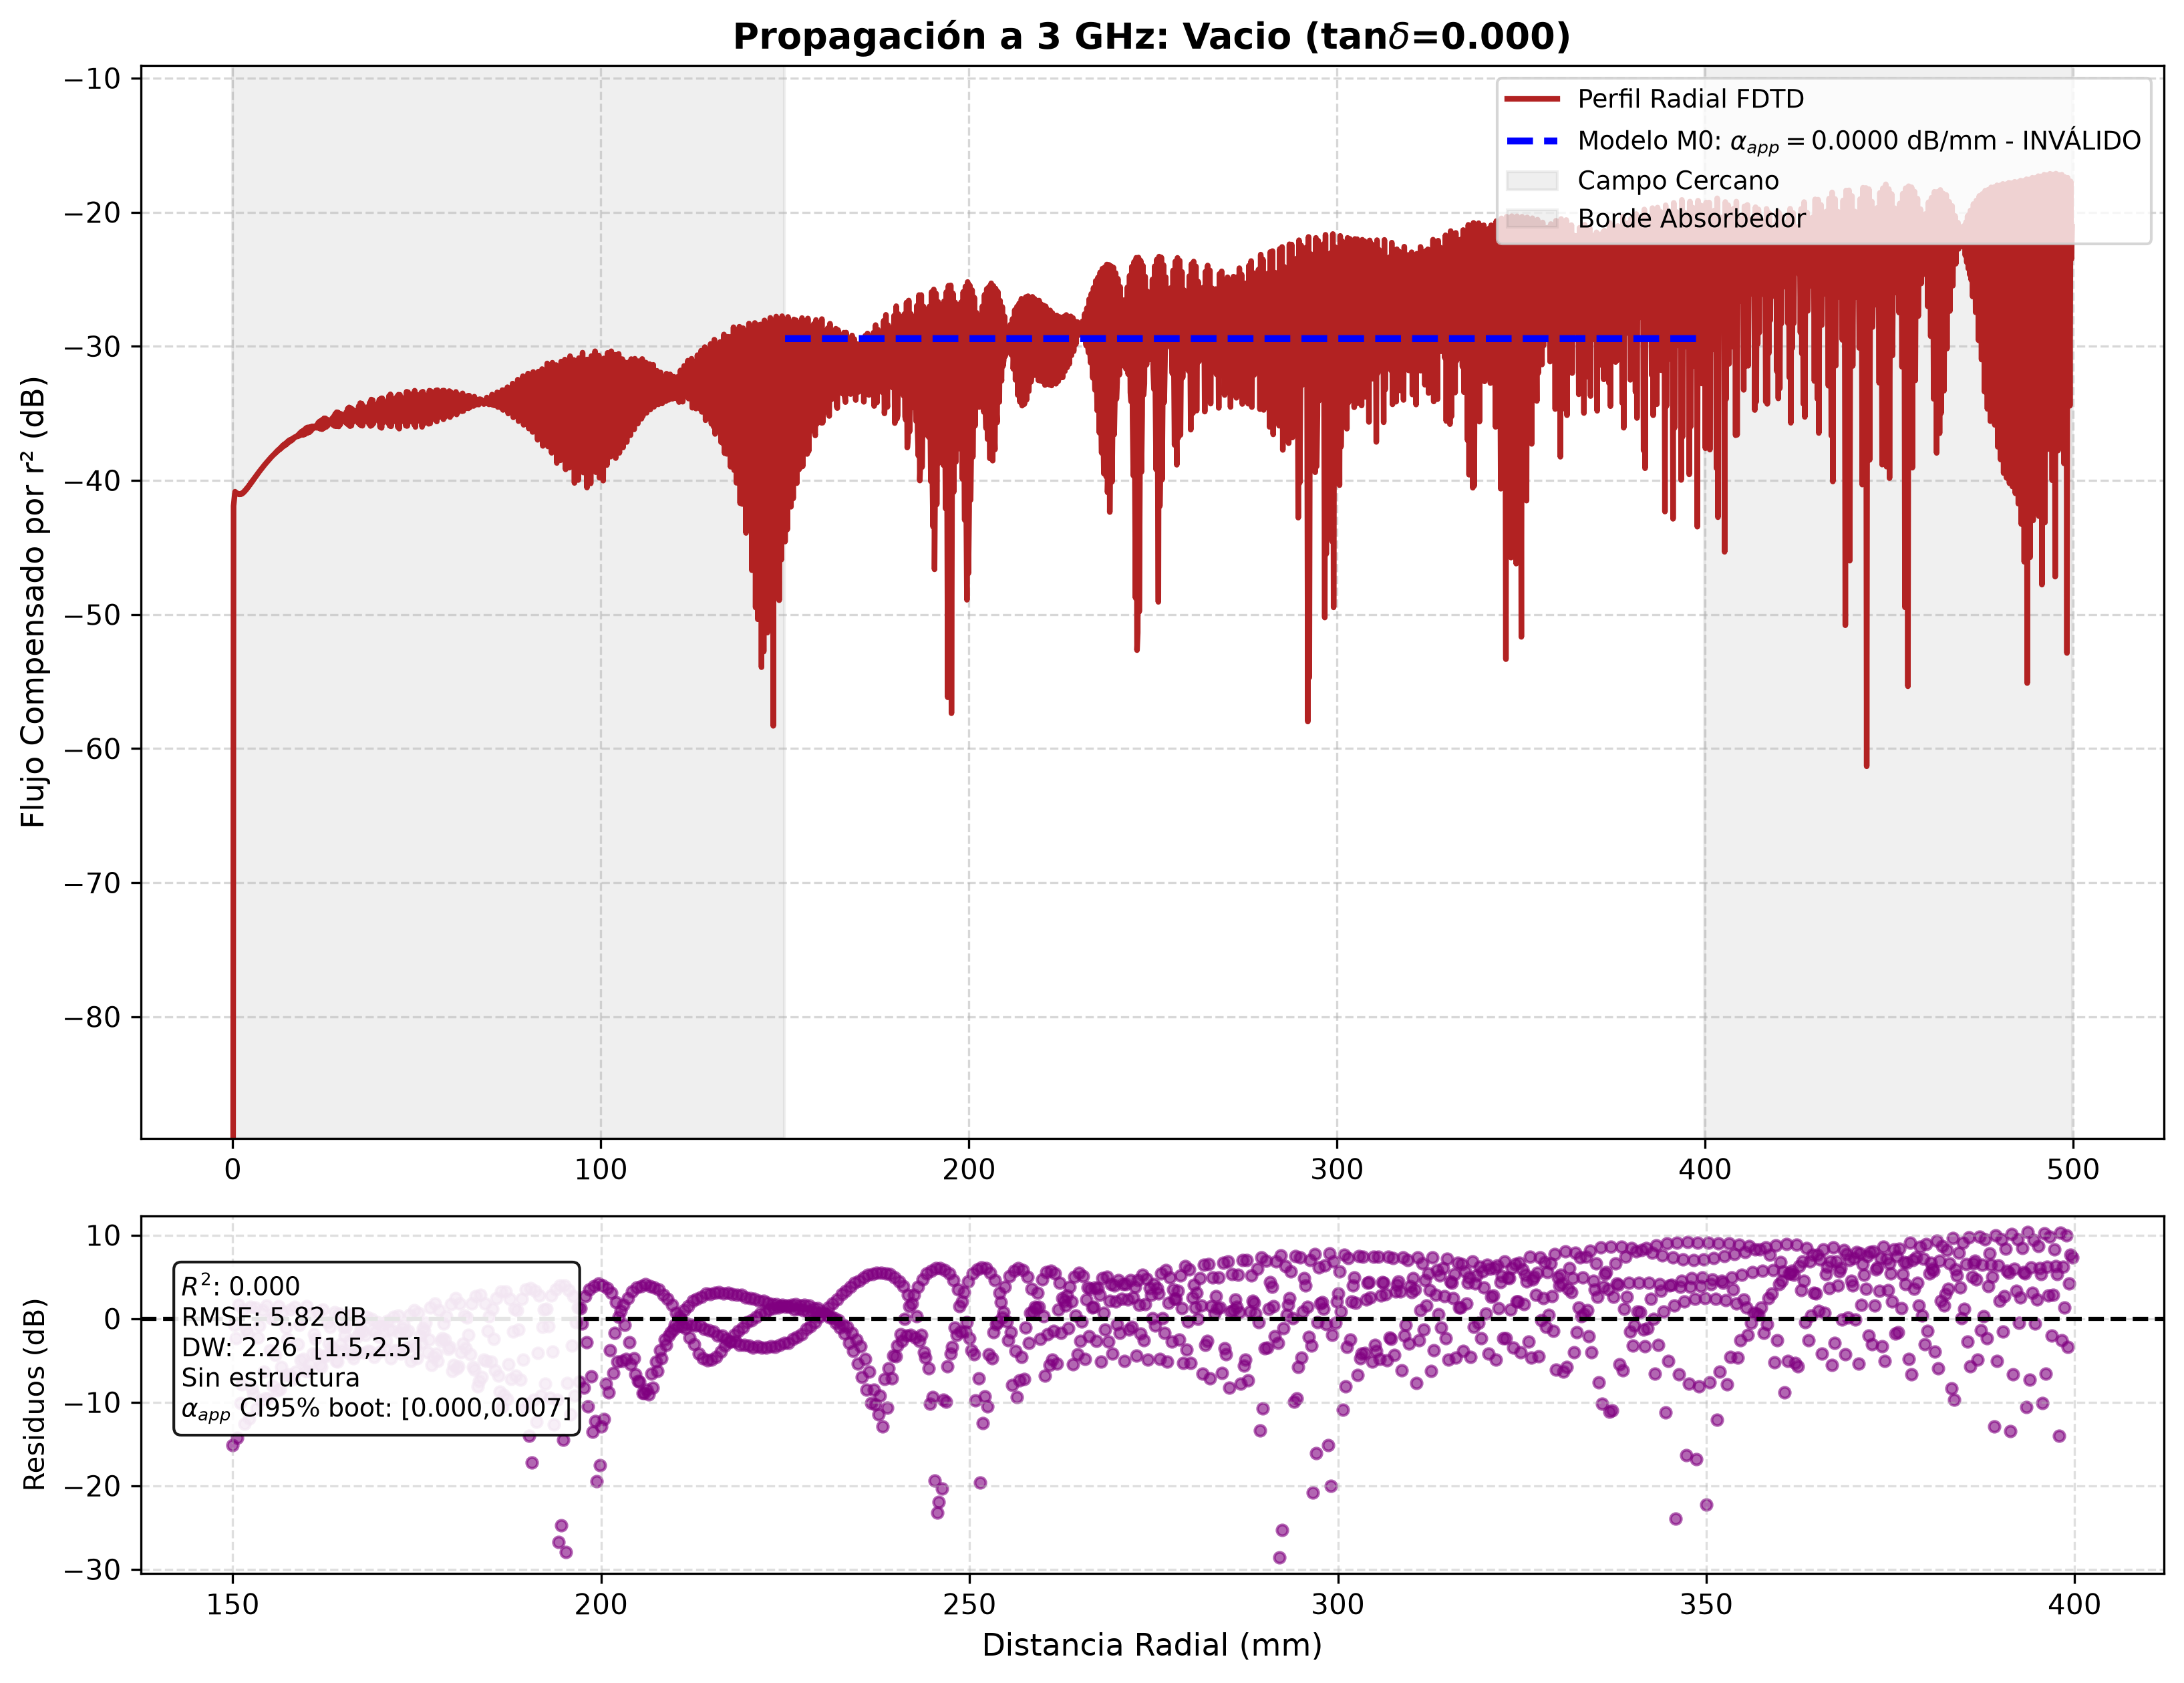
\includegraphics[width=0.81\linewidth]{figuras/Tesis_Resultado_vacio5px.png}\par\smallskip
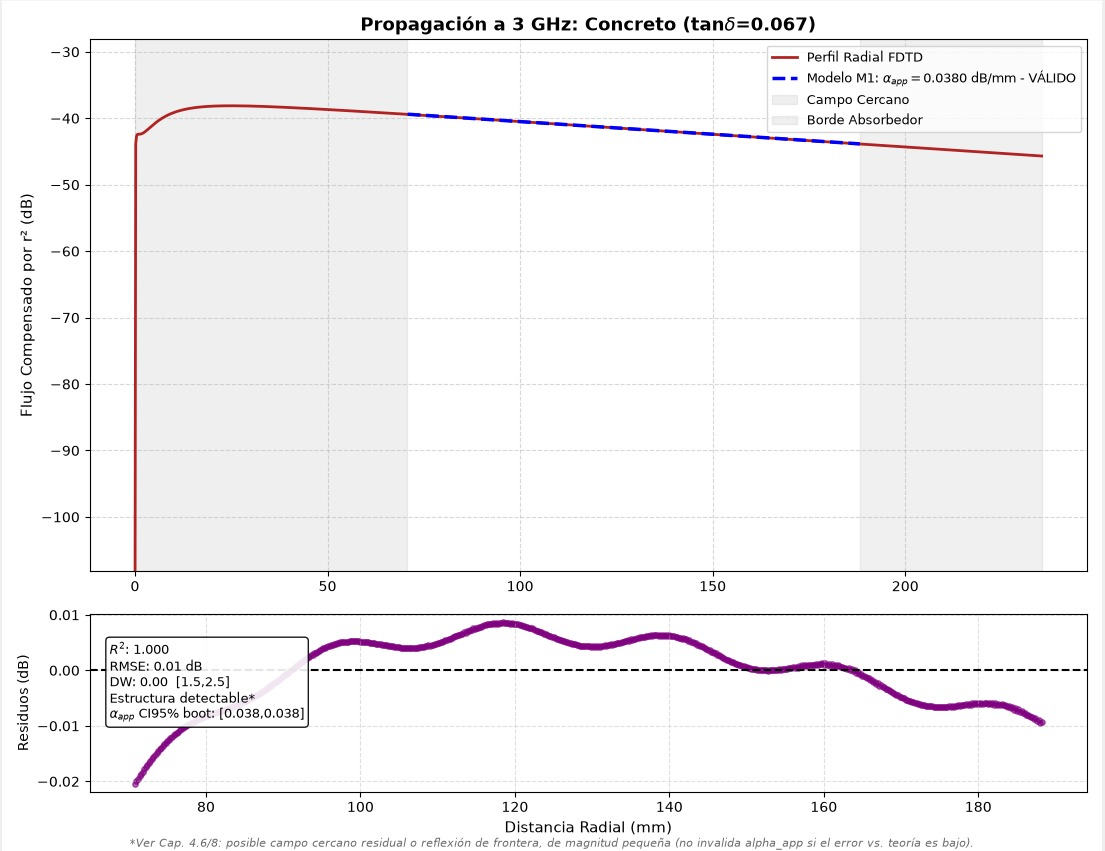
\includegraphics[width=0.81\linewidth]{figuras/Tesis_Resultado_concreto5px.jpeg}
\caption{Perfiles radiales y residuos a 5 px/mm en vacío (arriba) y concreto (abajo). Cada panel conservó su escala vertical.}\label{fig:perfiles-vacio-concreto}\end{figure}

\begin{figure}[htbp]\centering
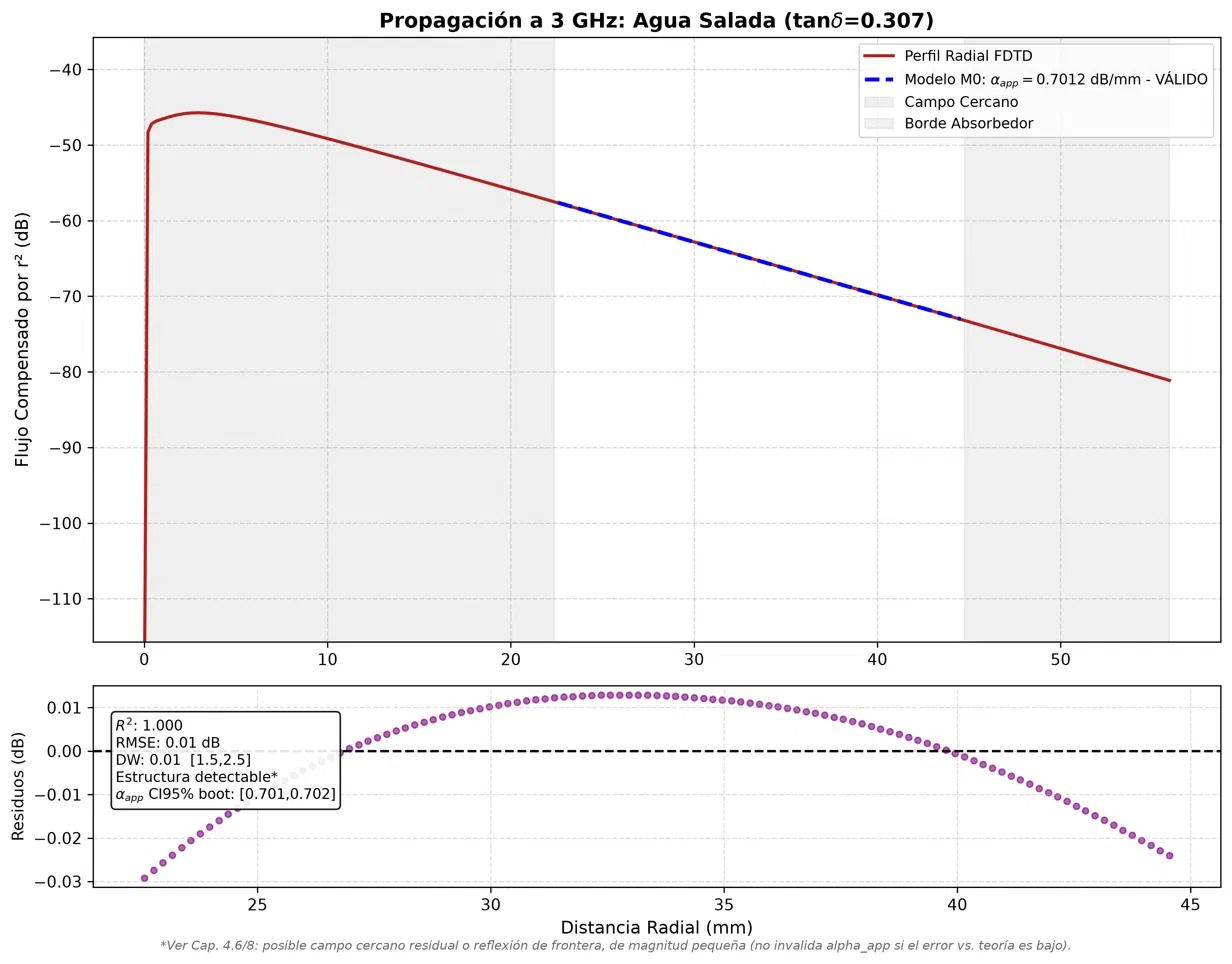
\includegraphics[width=0.81\linewidth]{figuras/Tesis_Resultado_agua_salada5px.jpeg}\par\smallskip
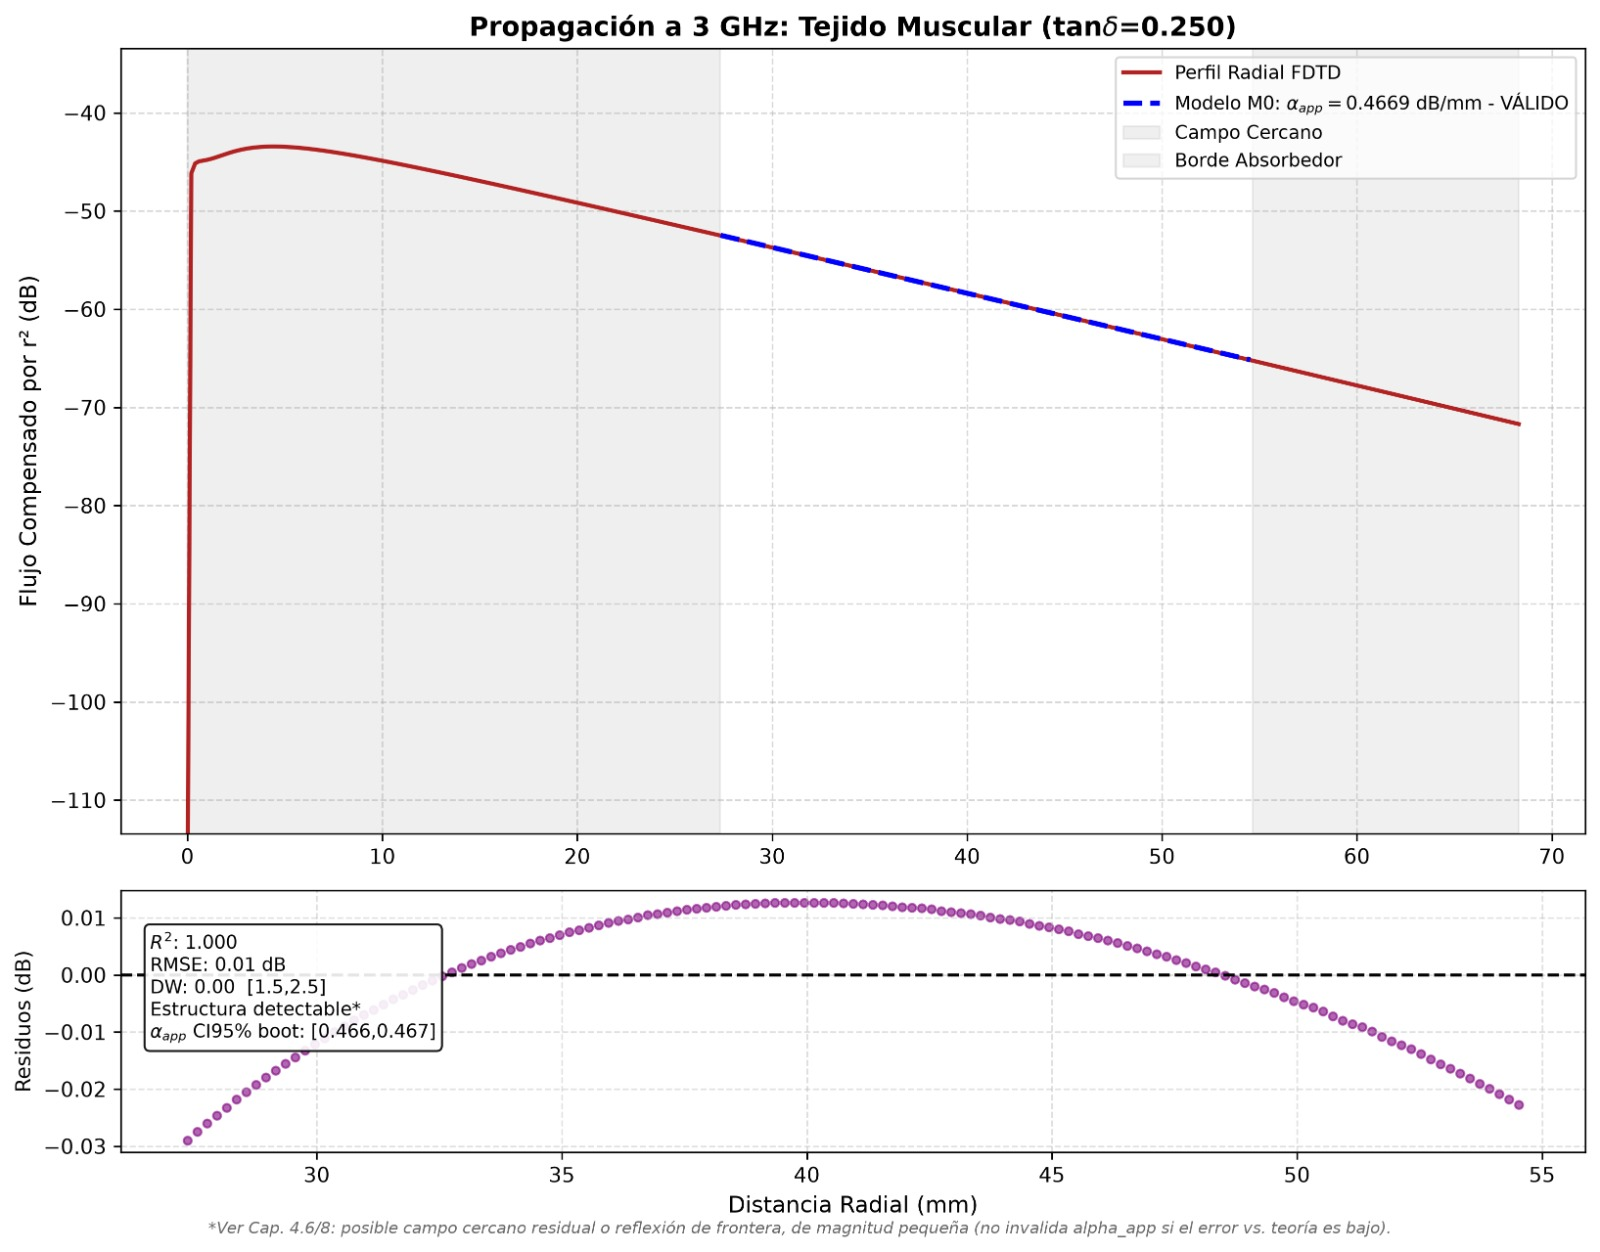
\includegraphics[width=0.81\linewidth]{figuras/Tesis_Resultados_Tejido_Muscular5px.jpeg}
\caption{Perfiles radiales y residuos a 5 px/mm en agua salada (arriba) y tejido muscular (abajo).}\label{fig:perfiles-agua-musculo}\end{figure}

\section{Efecto del refinamiento de malla}
Se examinó la evolución de la pendiente al reducir el paso espacial $h=1/R$, donde $R$ se expresó en px/mm y $h$ en mm. El Cuadro~\ref{tab:fdtd-mallas} reunió las seis corridas adicionales. Los intervalos conservaron la precisión del archivo de origen. En concreto a 10 px/mm ambos extremos coincidieron al redondearse a cuatro decimales.
\begin{table}[htbp]\centering\small\caption{Atenuación e incertidumbre del ajuste en las mallas adicionales.}\label{tab:fdtd-mallas}
\begin{tabular}{lccc}\hline Medio & $R$ (px/mm) & $\alpha_{\mathrm{app}}$ (dB/mm) & IC del 95\,\% (dB/mm) \\ \hline
Agua salada & 10 & 0.7133 & $[0.7130,0.7136]$ \\ & 20 & 0.7224 & $[0.7222,0.7226]$ \\ & 40 & 0.7267 & $[0.7267,0.7268]$ \\
Tejido muscular & 10 & 0.4778 & $[0.4776,0.4780]$ \\ & 20 & 0.4843 & $[0.4842,0.4845]$ \\
Concreto & 10 & 0.0381 & $[0.0381,0.0381]$ \\ \hline\end{tabular}\end{table}

En agua salada, los incrementos sucesivos de la pendiente fueron 0.0121, 0.0091 y 0.0043 dB/mm al duplicarse la resolución. La estimación a 5 px/mm difirió en 3.51\,\% de la obtenida a 40 px/mm. La última estimación quedó a 0.81\,\% del valor teórico. El orden aparente $p=\log_2(|\alpha_{2R}-\alpha_R|/|\alpha_{4R}-\alpha_{2R}|)$ cambió de 0.41 a 1.08 entre los dos tríos de mallas. Además, la selección del modelo pasó de M0 a M1 entre 10 y 20 px/mm. Se observó, por tanto, una aproximación monótona con incrementos decrecientes, aunque la variación del orden y del modelo limitó la interpretación de una extrapolación al continuo. Se reportó la diferencia entre mallas como medida empírica de sensibilidad.

En tejido muscular, el paso de 5 a 10 px/mm elevó la atenuación de 0.4669 a 0.4778 dB/mm. A 20 px/mm se obtuvo 0.4843 dB/mm. La diferencia entre las mallas extremas representó 3.59\,\% del valor más fino. La selección del ajuste también cambió de M0 a M1 en la malla más fina. En concreto, las pendientes a 5 y 10 px/mm difirieron aproximadamente en 0.26\,\% respecto de la segunda, según los valores redondeados. Para el vacío sólo se dispuso de una resolución, por lo que quedó indeterminado el error de discretización.

\subsection{Alcance de la resolución común}
A 5 px/mm se obtuvo un paso de 0.2 mm. Las longitudes de onda registradas correspondieron aproximadamente a 500 celdas en vacío, 235 en concreto, 56 en agua salada y 68 en músculo. En cambio, el diámetro de 0.4 mm del monopolo ocupó apenas dos celdas. La malla común permitió comparar los cuatro medios bajo la misma discretización geométrica. Su alcance quedó cuantificado para la atenuación por las diferencias frente a las mallas más finas disponibles. Estas diferencias fueron específicas de cada medio y también recogieron el efecto de la selección del ajuste.

Las restricciones de hardware limitaron los refinamientos, en particular en los dominios de mayor longitud de onda. Se utilizó una malla cilíndrica axisimétrica en las coordenadas $r$ y $z$, con modo azimutal $m=0$. Para un dominio físico fijo, al duplicarse la resolución se cuadruplicó aproximadamente el número de celdas. A igual factor de Courant y duración física, también se duplicó el número de pasos temporales, de modo que el número total de actualizaciones aumentó aproximadamente por un factor de ocho. Estas relaciones describieron el costo esperado. Los archivos históricos de atenuación carecieron de registros de memoria máxima y tiempo de ejecución por corrida. La campaña adicional de balance incorporó estas mediciones (Cuadro~\ref{tab:balance-costo}).

\section{Identificación de las corridas de balance}
Se utilizó el prefijo B para identificar una corrida de balance. Las letras AS, VA, CO y TM correspondieron a agua salada, vacío, concreto y tejido muscular. Los números 05 y 10 indicaron la resolución en px/mm. Así, B-AS05 designó agua salada a 5 px/mm y B-AS10, agua salada a 10 px/mm. B-VA05, B-CO05 y B-TM05 identificaron los otros tres medios a 5 px/mm. El índice del Anexo~\ref{an:balance-registros} vinculó estas abreviaturas con los archivos completos.

Las potencias tabuladas se expresaron como valores normalizados $P/P_*$, donde $P_*=E_*^2a^2/Z_0$ y $a=1$ mm. La escala de campo $E_*$ quedó pendiente de calibración. Los tiempos de simulación se expresaron en unidades de $a/c=3.33564$ ps. Las conversiones y la conductividad normalizada se definieron en la Sección~\ref{sec:unidades-campana}.

\section{Balance energético local en agua salada a 5 px/mm}\label{sec:balance-agua-cinco}
Se realizó una corrida adicional a 3 GHz para medir el flujo con signo y la disipación de Joule en una misma región. Se seleccionó un volumen anular de agua salada sin fuentes ni metal, comprendido entre $r=\lambda$ y $2\lambda$ y entre $z=0.25\lambda$ y $1.25\lambda$, donde $\lambda=11.187$ mm. Se sincronizaron los campos eléctrico y magnético y se integró el flujo con el factor de superficie cilíndrico correspondiente a cada cara. La potencia disipada se obtuvo independientemente mediante la integración volumétrica de la densidad de pérdida óhmica.

\begin{table}[htbp]\centering\small
\caption{Potencias del balance en el anillo de agua salada, normalizadas por $P_*$. Las muestras correspondieron a $t_1=1740.3$ y $t_2=1840.3$ en unidades temporales de Meep. Se indicaron magnitudes y sentido del flujo por separado.}\label{tab:balance-agua-cinco}
\begin{tabular}{lrr}\hline
Término & Primera muestra & Segunda muestra \\ \hline
Pared interior (entrada) & $1.239894\times10^{-5}$ & $1.239894\times10^{-5}$ \\
Tapa inferior (entrada) & $2.918001\times10^{-6}$ & $2.918001\times10^{-6}$ \\
Pared exterior (salida) & $2.000278\times10^{-6}$ & $2.000280\times10^{-6}$ \\
Tapa superior (salida) & $8.755799\times10^{-7}$ & $8.755806\times10^{-7}$ \\
Disipación de Joule & $1.243268\times10^{-5}$ & $1.243268\times10^{-5}$ \\
Residuo & $8.396156\times10^{-9}$ & $8.392715\times10^{-9}$ \\ \hline
\end{tabular}\end{table}

Se sumaron los flujos netos de las dos caras de entrada para obtener $P_{\rm ent}$ y los de las dos caras de salida para obtener $P_{\rm sal}$. El residuo se calculó mediante $R=P_{\rm ent}-P_{\rm sal}-P_{\rm J}$. En la segunda muestra, la disipación representó el 81.1695\,\% de $P_{\rm ent}$ y el flujo saliente, el 18.7757\,\%. El residuo relativo $100R/P_{\rm ent}$ pasó de 0.054816\,\% a 0.054794\,\% entre ambas muestras. Al normalizarlo exclusivamente por la entrada de la pared interior, tal como se registró en el archivo de la corrida, se obtuvo 0.067689\,\% en la segunda muestra.

Durante el intervalo de aproximadamente un período, el mayor cambio relativo entre las cuatro potencias de cara y la disipación fue de 0.000107\,\% respecto de la primera muestra del mismo término. Se registraron 157.3 s de ejecución y un máximo de 178.6 MiB de memoria residente del proceso en Ubuntu bajo WSL, con un procesador AMD Ryzen 5 4600H y un hilo de cómputo. Estas mediciones correspondieron a la corrida B-AS05. Posteriormente se completaron los balances B-VA05, B-CO05 y B-TM05 para los otros tres medios y B-AS10 para agua salada a 10 px/mm.

\section{Comparación del balance en los cuatro medios}\label{sec:balance-comparativo}
Se completó la misma medición anular en cada medio a 5 px/mm. Se conservaron los límites $r\in[\lambda,2\lambda]$ y $z\in[0.25\lambda,1.25\lambda]$, de modo que el volumen físico cambió con la longitud de onda. Se calculó la densidad media de flujo mediante $S_r=-\operatorname{Re}(E_zH_\phi^*)/2$ y $S_z=\operatorname{Re}(E_rH_\phi^*)/2$. La pérdida se integró como
\begin{equation}
 P_{\rm J}=\int_{\lambda}^{2\lambda}\int_{0.25\lambda}^{1.25\lambda}
 \frac{\varepsilon_r\sigma_D}{2}\left(|E_r|^2+|E_z|^2\right)2\pi r\, dz\,dr,
 \label{eq:joule-anular}
\end{equation}
donde $\sigma_D$ correspondió a la conductividad del término de evolución de $D$ en unidades de Meep. Se empleó cuadratura trapezoidal con paso de muestreo igual o inferior a una celda. El factor $2\pi r$ se incorporó explícitamente tanto en el volumen como en las superficies correspondientes.

Se orientaron hacia fuera las normales de las cuatro caras y se denotaron sus flujos netos por $F_j$. Con esta convención se obtuvieron
\begin{equation}
 P_{\rm ent}=-\sum_j\min(F_j,0),\qquad
 P_{\rm sal}=\sum_j\max(F_j,0),\qquad
 \eta_{\rm J}=\frac{P_{\rm J}}{P_{\rm ent}},\qquad
 \delta_{\rm B}=\frac{P_{\rm ent}-P_{\rm sal}-P_{\rm J}}{P_{\rm ent}}.
 \label{eq:balance-normalizado}
\end{equation}
La agrupación por signo se efectuó sobre el flujo integrado de cada cara. Las potencias se expresaron en unidades de Meep y las fracciones se normalizaron por la entrada neta total al anillo. El Cuadro~\ref{tab:balance-medios} presentó la segunda muestra de cada corrida. Los identificadores remitieron a los archivos individuales del \hyperref[an:balance-registros]{Anexo A}.

\begin{table}[htbp]\centering\small
\caption{Balance local a 5 px/mm. Las tres últimas columnas se expresaron como porcentajes de $P_{\rm ent}$ y su suma fue 100, dentro del redondeo. El residuo conservó su signo.}\label{tab:balance-medios}
\begin{tabular}{llrrrr}\hline
Medio & ID & $P_{\rm ent}/P_*$ & Disipada & Saliente & Residuo \\ \hline
Vacío & B-VA05 & $1.094598\!\times\!10^{-3}$ & 0.0000 & 99.9861 & 0.013943 \\
Concreto & B-CO05 & $3.686265\!\times\!10^{-4}$ & 30.3782 & 69.6198 & 0.002011 \\
Agua salada & B-AS05 & $1.531694\!\times\!10^{-5}$ & 81.1695 & 18.7757 & 0.054794 \\
Músculo & B-TM05 & $3.819407\!\times\!10^{-5}$ & 74.5328 & 25.4343 & 0.032973 \\ \hline
\end{tabular}\end{table}

En los cuatro medios, la pared interior y la tapa inferior aportaron potencia al anillo, mientras que la pared exterior y la tapa superior registraron salida. Se obtuvo la mayor fracción disipada en agua salada, seguida del músculo y del concreto. En vacío, $P_{\rm J}=0$ se siguió directamente de la conductividad nula asignada. La entrada y la salida concordaron dentro del residuo informado. Las potencias absolutas correspondieron a la amplitud numérica de excitación utilizada y su conversión a vatios quedó condicionada a una calibración de la fuente.

\subsection{Variación entre las dos muestras temporales}
Se registraron dos muestras separadas aproximadamente por un período de la fuente, después del tiempo de estabilización del simulador. Para comparar los medios con una normalización común se definió
\begin{equation}
 \Delta_{\rm t}=\frac{\max_k|Q_k(t_2)-Q_k(t_1)|}{P_{\rm ent}(t_2)},
 \label{eq:variacion-temporal}
\end{equation}
donde $Q_k$ recorrió las cuatro potencias de cara y $P_{\rm J}$. Se incluyeron por separado ambos residuos en el Cuadro~\ref{tab:balance-tiempo}.

\begin{table}[htbp]\centering\small
\caption{Comprobación temporal del balance. Los tiempos se expresaron en unidades de Meep y las tres últimas columnas en porcentaje. $\delta_{\rm B}$ se normalizó por la entrada de su propia muestra.}\label{tab:balance-tiempo}
\begin{tabular}{lrrrrr}\hline
ID & $t_1$ & $t_2$ & $100\delta_{\rm B}(t_1)$ & $100\delta_{\rm B}(t_2)$ & $100\Delta_{\rm t}$ \\ \hline
B-VA05 & 3497.60 & 3597.60 & 0.000308 & 0.013943 & 0.017448 \\
B-CO05 & 3496.80 & 3596.80 & 0.001772 & 0.002011 & 0.000143 \\
B-AS05 & 1740.30 & 1840.30 & 0.054816 & 0.054794 & 0.000014 \\
B-TM05 & 1743.10 & 1843.10 & 0.032984 & 0.032973 & 0.000005 \\
B-AS10 & 1740.30 & 1840.25 & 0.021675 & 0.021640 & 0.000021 \\ \hline
\end{tabular}\end{table}

Los términos variaron menos de 0.000144\,\% de la entrada final en los medios con pérdidas. En vacío se observó una variación mayor, de 0.017448\,\%, y el residuo aumentó durante el último intervalo. La comprobación quedó limitada a dos instantes de fase aproximadamente equivalente. La ausencia de una serie temporal extensa dejó sin cuantificar el almacenamiento residual de energía y la estabilidad a tiempos mayores.

\subsection{Sensibilidad del balance de agua salada al refinamiento}
Se repitió la integración en el mismo anillo físico a 10 px/mm. Se obtuvo $P_{\rm ent}=1.073782\times10^{-5}$ y $P_{\rm J}=8.679552\times10^{-6}$ en unidades de Meep. La fracción disipada pasó de 81.1695\,\% a 80.8316\,\%, la fracción saliente alcanzó 19.1468\,\% y el residuo descendió a 0.021640\,\%. La reducción de la fracción disipada fue de 0.337943 puntos porcentuales, equivalente al 0.418083\,\% de la fracción obtenida con la malla fina.

La entrada absoluta disminuyó 29.8958\,\% y la disipación absoluta, 30.1876\,\%, respecto de la malla de 5 px/mm. La normalización compensó gran parte de esta variación común. Por ello, la sensibilidad de 0.4181\,\% caracterizó específicamente el cociente $\eta_{\rm J}$. Dos resoluciones proporcionaron una diferencia observada entre mallas, mientras que la estimación del orden de convergencia del balance y de su error al continuo quedó pendiente. Para concreto, músculo y vacío se contó con una sola malla de balance.

Los resultados de balance se acompañaron de sus residuos, variaciones temporales y, en agua salada, de la diferencia entre mallas. Estos diagnósticos describieron fuentes distintas de discrepancia numérica. La disponibilidad de dos muestras deterministas dejó sin estimar una incertidumbre estadística del balance. Los IC del ajuste de atenuación se mantuvieron asociados exclusivamente a aquella extracción.

\clearpage
\subsection{Costo computacional medido}\label{sec:costo-balance}
Las cuatro corridas adicionales se ejecutaron secuencialmente mediante tareas de VS Code conectado a Ubuntu bajo WSL2. Se utilizó un procesador AMD Ryzen 5 4600H, con un hilo OpenMP y uno OpenBLAS por proceso. El entorno dispuso de 7.44 GiB de memoria total. Se emplearon Python 3.13.13, NumPy 2.4.3 y Meep 1.33.0-beta. El Cuadro~\ref{tab:balance-costo} incluyó también la corrida B-AS05 previamente completada.

\begin{table}[htbp]\centering\small
\caption{Tiempo de pared y memoria residente máxima de cada proceso de balance. El tiempo incluyó inicialización, avance temporal, extracción e integración.}\label{tab:balance-costo}
\begin{tabular}{lrrr}\hline
ID & Resolución (px/mm) & Tiempo (s) & RSS máxima (MiB) \\ \hline
B-VA05 & 5 & 26977.1 & 4868.2 \\
B-CO05 & 5 & 6491.7 & 1326.1 \\
B-AS05 & 5 & 157.3 & 178.6 \\
B-TM05 & 5 & 300.3 & 213.2 \\
B-AS10 & 10 & 1581.1 & 384.3 \\ \hline
\end{tabular}\end{table}

El vacío requirió 7.49 h y 4.75 GiB de RSS máxima, mientras que el concreto requirió 1.80 h. En agua salada, duplicar la resolución elevó el tiempo por un factor de 10.05 y la RSS por un factor de 2.15. Estos cocientes describieron las ejecuciones medidas y dependieron también de los costos fijos y de la actividad del sistema. El escalado cuadrático ideal de memoria aplicado al vacío a 10 px/mm habría supuesto aproximadamente 19 GiB, por encima de la memoria disponible en WSL. Esta proyección se distinguió del consumo efectivamente medido y sustentó la restricción práctica de la comparación común a 5 px/mm.


\section{Verificación de propagación uniforme}\label{sec:resultados-planar}
La campaña VP comprendió ocho corridas independientes de la antena. En los medios disipativos, los errores de atenuación respecto de la solución analítica fueron inferiores a 0.16\,\% a 5 px/mm y a 0.041\,\% a 10 px/mm (Cuadro~\ref{tab:planar}). En vacío se obtuvieron pendientes de $-2.80\times10^{-11}$ y $2.01\times10^{-10}$ dB/mm, compatibles con cero dentro de sus IC. Al ser nula la referencia, se informó la diferencia absoluta y se omitió el error relativo.

\begin{table}[htbp]\centering\footnotesize
\caption{Verificación planar: atenuación e IC condicional del 95\,\% en dB/mm. El error relativo se calculó respecto de la solución analítica. Las cifras adicionales permitieron distinguir el IC del error sistemático.}\label{tab:planar}
\begin{tabular}{lrrr}\hline
ID & $\alpha_{\rm VP}$ & IC del ajuste & Error (\%) \\ \hline
VP-VA05 & $-2.80\times10^{-11}$ & $[-6.61\times10^{-8},\,6.53\times10^{-8}]$ & --- \\
VP-VA10 & $2.01\times10^{-10}$ & $[-2.01\times10^{-8},\,2.14\times10^{-8}]$ & --- \\
VP-CO05 & $0.038546428$ & $[0.038546315,\,0.038546532]$ & 0.0095 \\
VP-CO10 & $0.038543997$ & $[0.038543964,\,0.038544028]$ & 0.0032 \\
VP-AS05 & $0.733774319$ & $[0.733756741,\,0.733792172]$ & 0.1575 \\
VP-AS10 & $0.732914311$ & $[0.732911332,\,0.732917661]$ & 0.0401 \\
VP-TM05 & $0.492580649$ & $[0.492576832,\,0.492584230]$ & 0.1060 \\
VP-TM10 & $0.492193312$ & $[0.492191869,\,0.492194743]$ & 0.0273 \\
\hline\end{tabular}\end{table}

La variación temporal máxima del flujo fue inferior a $7.87\times10^{-6}$ en vacío y a $2.95\times10^{-10}$ en los medios disipativos. Los RMSE fueron menores que $1.4\times10^{-5}$ dB en vacío. La Figura~\ref{fig:planar} mostró las diferencias espaciales respecto del perfil analítico, normalizado en el primer punto; las oscilaciones y la deriva restante disminuyeron al refinar la malla en los medios con pérdidas.

\begin{figure}[!htbp]\centering
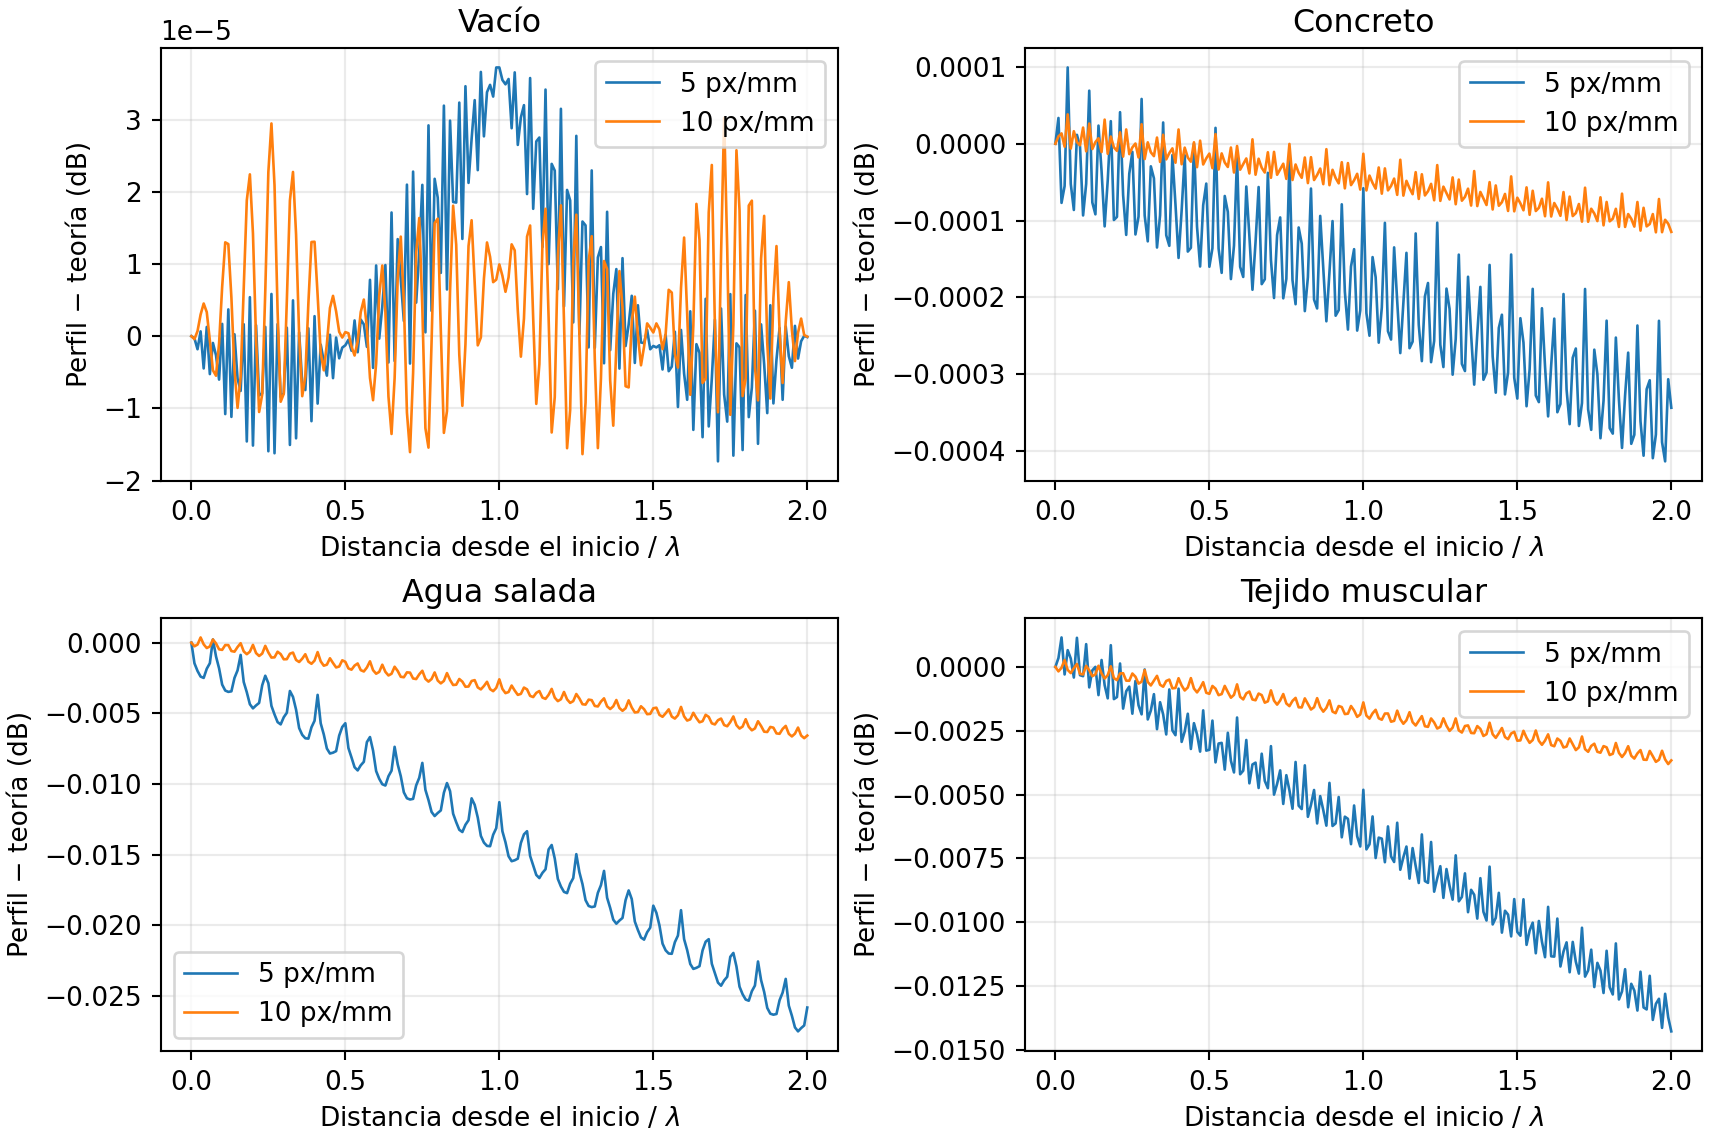
\includegraphics[width=\textwidth]{figuras/verificacion_onda_plana.png}
\caption{Diferencia entre el perfil planar normalizado y la predicción analítica. Cada panel utilizó su propia escala vertical. Se compararon las dos mallas sobre la misma ventana física de cada medio.}\label{fig:planar}
\end{figure}

Una ejecución inicial con encendido abrupto produjo, en vacío a 5 px/mm, un RMSE de 1.13 dB y un cambio temporal del flujo de 0.679. Se descartó como comprobación estacionaria y se conservó como diagnóstico. El cambio de activación redujo ambas discrepancias en esta prueba; los registros originales de la antena permanecieron separados. Se archivaron las dieciséis ejecuciones, sus perfiles y las dos versiones del verificador.

Las ocho corridas con activación suave acumularon 17.9 s de tiempo medido y una RSS máxima del proceso de 111.2 MiB. Se ejecutaron secuencialmente desde VS Code en Ubuntu con un solo hilo. La RSS fue acumulativa dentro del proceso; no se interpretó como el consumo independiente de cada caso.
